% flock paper skeleton. Figures and tables under figures/ are regenerated by
%   uv run flock analyze <run-id> --paper
% Build: pdflatex main.tex (twice) or latexmk -pdf main.tex
\documentclass[11pt]{article}
\usepackage[margin=1in]{geometry}
\usepackage{graphicx}
\usepackage{booktabs}
\usepackage{amsmath}
\usepackage{natbib}
\usepackage{hyperref}

% auto-generated by `flock analyze --paper`; do not edit by hand
\newcommand{\deltakappa}{0.488}
\newcommand{\deltakappaCIlow}{0.074}
\newcommand{\deltakappaCIhigh}{0.720}
\newcommand{\deltakappaP}{0.0028}


\title{Do LLM Trading Agents Converge?\\
\large Measuring strategy convergence and emergent coordination in
foundation-model market participants}
\author{Lewis Smith}
\date{\today}

\begin{document}
\maketitle

\begin{abstract}
% One paragraph: question, method (replay + shared exchange, matched
% baselines, pre-registered inference), headline result, implication.
Foundation models may become a common decision layer across market
participants. We measure whether cohorts of LLM trading agents converge on
similar strategies more than the infrastructure they may replace. Across
historical replay and a shared double-auction market, and against matched
classical-algorithm cohorts and empirical dispersion panels, we find
$\Delta\kappa = \deltakappa$ (95\% CI $[\deltakappaCIlow, \deltakappaCIhigh]$,
permutation $p = \deltakappaP$). % placeholder numbers from the latest run
\end{abstract}

\section{Introduction}
% Motivation: model monoculture -> correlated trading without communication.
% Contributions: (1) dispersion contrast with matched baselines, (2)
% pre-registered inference, (3) cross-provider design, (4) decision-log
% datasets for agents in finance.

\section{Related work}
% See docs/research/07-related-work.md: LSV/Sias herding; Calvano et al.
% algorithmic collusion; Khandani-Lo quant quake; outcome homogenization.

\section{Experimental design}
% Summarize docs/research/02-experimental-design.md: replay vs shared
% exchange topology; cohorts (LLM / baseline / null); identical information
% sets; controls; pre-registration (docs/research/06, tag prereg-v1).

\section{Metrics and inference}
% Summarize docs/research/03-metrics.md: decision / portfolio / strategy
% hierarchy; LSV, Sias, cascades; permutation tests with agent relabeling;
% BCa bootstrap; Holm-Bonferroni.

\section{Results}

\begin{table}[t]
\centering
% auto-generated by `flock analyze --paper`; do not edit by hand
% run exp-010-shared-exchange-s42-3eb5aaf9 (config 3eb5aaf9a937d197, git 9489505cb9)
\begin{tabular}{lrrrrr}
\toprule
Cohort & Cohen's $\kappa$ & Agreement & Overlap & Fingerprint disp. & LSV \\
\midrule
llm & 0.526 & 0.762 & 0.415 & 0.214 & 0.301 \\
baseline & 0.038 & 0.332 & 0.366 & 0.348 & -0.083 \\
null & -0.046 & 0.355 & 0.363 & 0.306 & -0.040 \\
\bottomrule
\end{tabular}

\caption{Within-cohort convergence by metric. Higher $\kappa$/overlap and
lower fingerprint dispersion indicate convergence; the null cohort gives the
chance floor.}
\label{tab:metrics}
\end{table}

\begin{figure}[t]
\centering
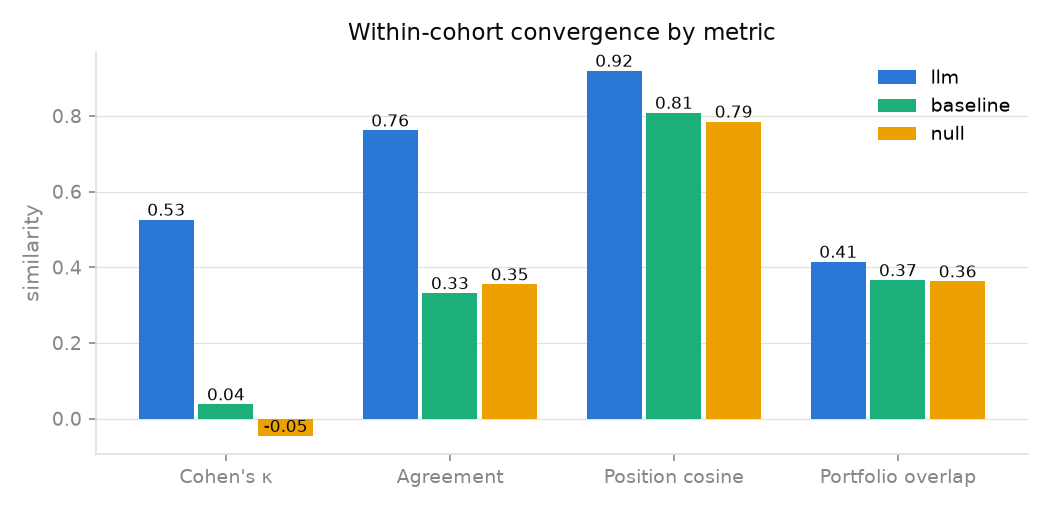
\includegraphics[width=\linewidth]{figures/convergence_by_cohort.png}
\caption{Within-cohort convergence by metric and cohort.}
\label{fig:convergence}
\end{figure}

\begin{figure}[t]
\centering
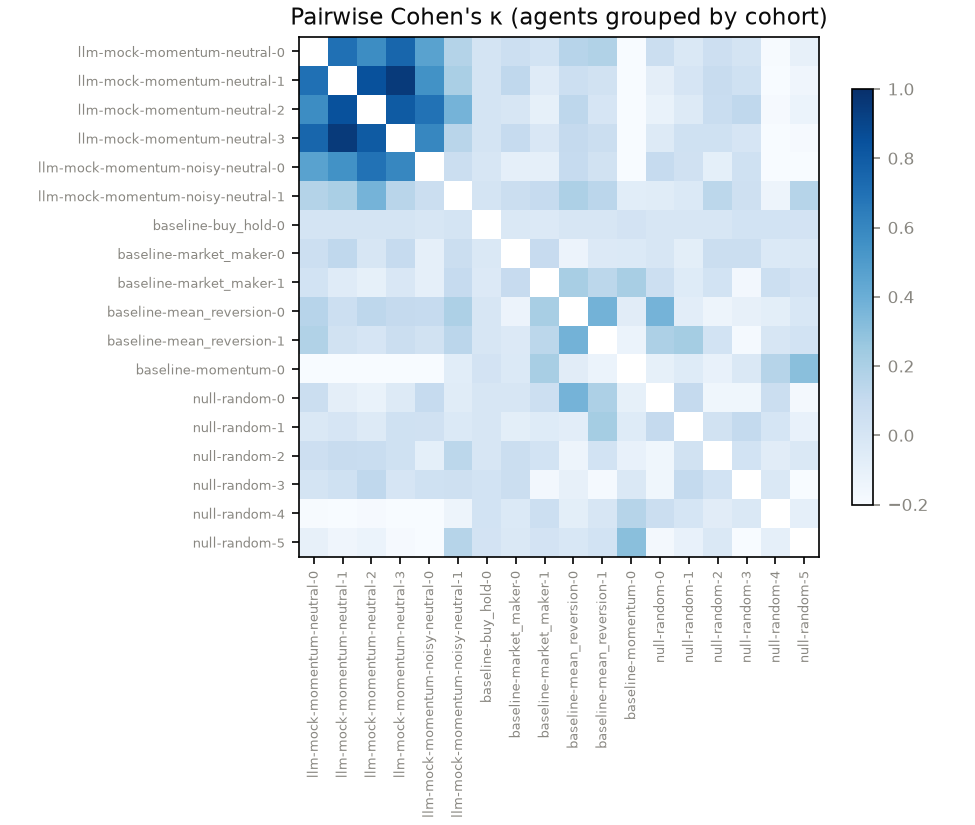
\includegraphics[width=0.8\linewidth]{figures/kappa_heatmap.png}
\caption{Pairwise Cohen's $\kappa$; block structure along the diagonal
indicates within-cohort convergence.}
\label{fig:heatmap}
\end{figure}

\begin{figure}[t]
\centering
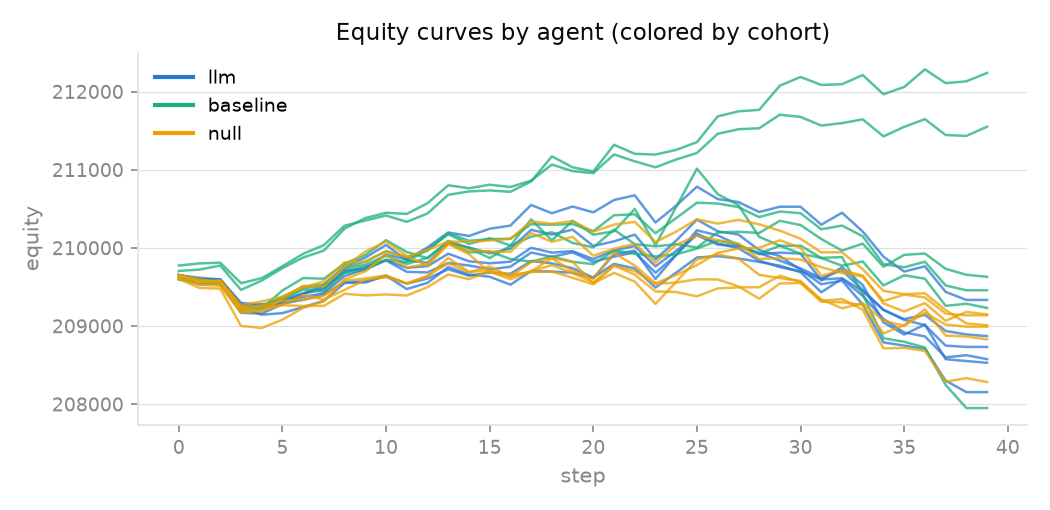
\includegraphics[width=\linewidth]{figures/equity_curves.png}
\caption{Equity curves by agent, colored by cohort.}
\label{fig:equity}
\end{figure}

\section{Discussion}
% Mechanisms (shared prior vs shared optimum), persona/information
% decorrelation trade-off, shared-market amplification (H5).

\section{Limitations}
% Contamination; prompt-template sensitivity (paraphrase battery); baseline
% representativeness; long-only markets; daily bars.

\section{Ethics and disclosure}
% No live trading; public data; systemic-risk framing; dataset release terms.

\bibliographystyle{plainnat}
% \bibliography{references}

\end{document}
